\hypertarget{historiadores-e-suxe9ries-temporais}{%
\chapter{Historiadores e Séries Temporais}\label{historiadores-e-suxe9ries-temporais}}

\section*{Objetivos de Aprendizagem}

Ao final deste capítulo, o leitor será capaz de:

\begin{itemize}
\tightlist
\item
  Distinguir tendência real de tendência histórica e dimensionar a janela de registro.
\item
  Reconhecer por que bancos relacionais convencionais não atendem à historização de processo.
\item
  Explicar o efeito da compressão por exceção e a consequência de configurá-la mal.
\item
  Definir política de retenção, agregação e descarte por classe de dado.
\item
  Separar histórico de processo de histórico de eventos e de trilha de auditoria.
\item
  Comparar soluções de historização pela função e pela limitação, sem apelo de fabricante.
\end{itemize}

\begin{center}\rule{0.5\linewidth}{0.5pt}\end{center}

\hypertarget{a-pergunta-que-o-histuxf3rico-responde}{%
\section{A pergunta que o histórico responde}\label{a-pergunta-que-o-histuxf3rico-responde}}

O histórico de processo atende a três públicos que fazem perguntas diferentes:

\begin{longtable}[]{@{}
  >{\raggedright\arraybackslash}p{(\columnwidth - 4\tabcolsep) * \real{0.3333}}
  >{\raggedright\arraybackslash}p{(\columnwidth - 4\tabcolsep) * \real{0.3333}}
  >{\raggedright\arraybackslash}p{(\columnwidth - 4\tabcolsep) * \real{0.3333}}@{}}
\toprule\noalign{}
\begin{minipage}[b]{\linewidth}\raggedright
Público
\end{minipage} & \begin{minipage}[b]{\linewidth}\raggedright
Pergunta
\end{minipage} & \begin{minipage}[b]{\linewidth}\raggedright
O que precisa ser preservado
\end{minipage} \\
\midrule\noalign{}
\endhead
\bottomrule\noalign{}
\endlastfoot
Operação & ``O que está acontecendo agora e nos últimos minutos?'' & Alta resolução no presente, com atualização contínua \\
Engenharia e manutenção & ``Por que parou, o que mudou antes da falha, qual a tendência da variável?'' & Resolução suficiente para reconstruir o transitório \\
Gestão e conformidade & ``Quanto produzimos, qual o consumo, como estava a emissão naquele dia?'' & Integridade, retenção longa e agregação confiável \\
\end{longtable}

As três exigências são incompatíveis entre si quando o armazenamento é tratado como um só. Guardar
tudo com máxima resolução por anos é caro; guardar tudo comprimido o suficiente para caber em disco
destrói a resposta que a engenharia precisa. Todo sistema de historização real é uma negociação
entre essas demandas --- e essa negociação é projeto, não parâmetro deixado no padrão.

\begin{center}\rule{0.5\linewidth}{0.5pt}\end{center}

\hypertarget{tenduxeancia-real-e-tenduxeancia-histuxf3rica}{%
\section{Tendência real e tendência histórica}\label{tenduxeancia-real-e-tenduxeancia-histuxf3rica}}

São dois objetos diferentes, com armazenamento diferente.

\begin{itemize}
\tightlist
\item
  A \textbf{tendência real} exibe os últimos valores em função do tempo, de forma dinâmica. Cada curva
  guarda os valores em um \textbf{vetor na memória} da estação de supervisão.
\item
  A \textbf{tendência histórica} recupera valores gravados em memória secundária (disco, SSD) e exibe o
  intervalo escolhido pelo operador. É estática, aceita mais variáveis e permite recuperar qualquer
  período.
\end{itemize}

\begin{figure}
\centering
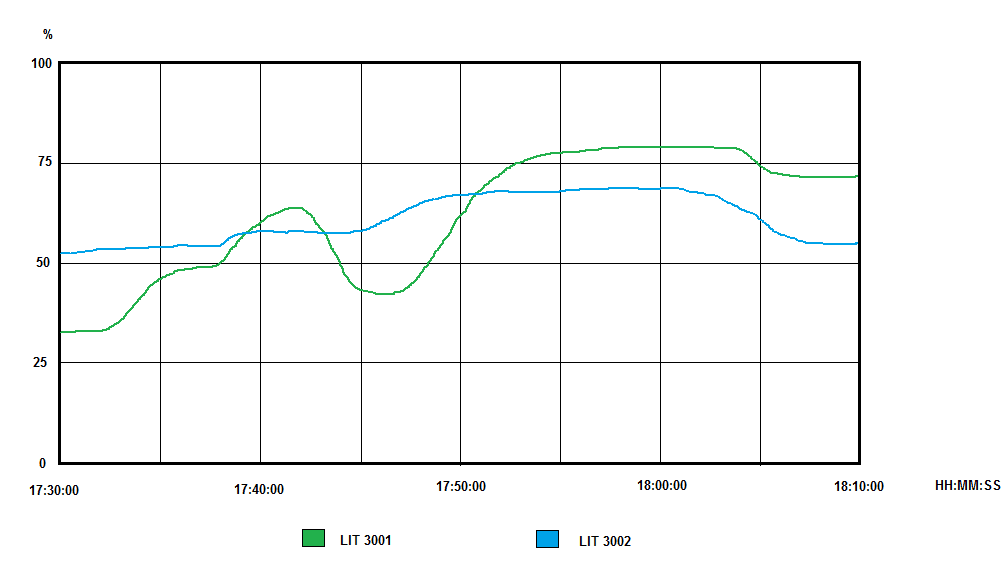
\includegraphics{../figuras/cap16-tendencia-real.png}
\caption[Figura 16.1 -- Tendência real com duas variáveis de nível, escala fixa e legenda]{Figura 16.1 -- Tendência real com duas variáveis de nível, escala fixa e legenda. \textbf{Fonte:} \emph{Livro SCADA --- versão para análise}, p.~67 (Machado, Pontes e Vianna, reproduzida com crédito).}
\end{figure}

Na tendência real, o tamanho do vetor é o recurso limitado, e a aritmética é implacável:

\begin{lstlisting}
janela de tempo = taxa de amostragem x numero de amostras

  100 ms x 1024 amostras = 102,4 s   (1,7 minuto)
  1 s    x 1024 amostras = 1024 s    (17 minutos)
  5 s    x 1024 amostras = 5120 s    (85 minutos)
  10 min / 5 s           = 120 amostras no vetor
\end{lstlisting}

Não existe configuração que amplie a janela e melhore a resolução ao mesmo tempo: aumentar uma
obriga a reduzir a outra, ou a ampliar memória. É por isso que a tendência real é organizada por
\textbf{grupos de variáveis com dinâmica parecida} --- vazão e pressão em um grupo, temperatura de mancal
em outro.

\textbf{Tabela 16.1 -- Tendência real \ensuremath{\times} tendência histórica}

\begin{longtable}[]{@{}
  >{\raggedright\arraybackslash}p{(\columnwidth - 4\tabcolsep) * \real{0.3333}}
  >{\raggedright\arraybackslash}p{(\columnwidth - 4\tabcolsep) * \real{0.3333}}
  >{\raggedright\arraybackslash}p{(\columnwidth - 4\tabcolsep) * \real{0.3333}}@{}}
\toprule\noalign{}
\begin{minipage}[b]{\linewidth}\raggedright
Aspecto
\end{minipage} & \begin{minipage}[b]{\linewidth}\raggedright
Tendência real
\end{minipage} & \begin{minipage}[b]{\linewidth}\raggedright
Tendência histórica
\end{minipage} \\
\midrule\noalign{}
\endhead
\bottomrule\noalign{}
\endlastfoot
Armazenamento & Memória RAM da estação & Disco rígido, SSD ou servidor de histórico \\
Comportamento & Dinâmica, atualizada continuamente & Estática, recuperada sob consulta \\
Janela & Limitada pelo tamanho do vetor & Limitada pela política de retenção \\
Número de variáveis & Normalmente poucas (1 a 8 penas por gráfico) & Muitas, com filtro por grupo e período \\
Perda ao reiniciar & Sim: o vetor é volátil & Não: o dado está gravado \\
Uso típico & Acompanhar a operação corrente & Diagnosticar, comparar, relatar, auditar \\
\end{longtable}

\begin{center}\rule{0.5\linewidth}{0.5pt}\end{center}

\hypertarget{os-paruxe2metros-que-decidem-o-que-vocuxea-vai-ver-depois}{%
\section{Os parâmetros que decidem o que você vai ver depois}\label{os-paruxe2metros-que-decidem-o-que-vocuxea-vai-ver-depois}}

Quatro parâmetros definem o resultado de um gráfico de tendência, e todos os quatro são decididos
muito antes de alguém precisar do histórico.

\begin{figure}
\centering
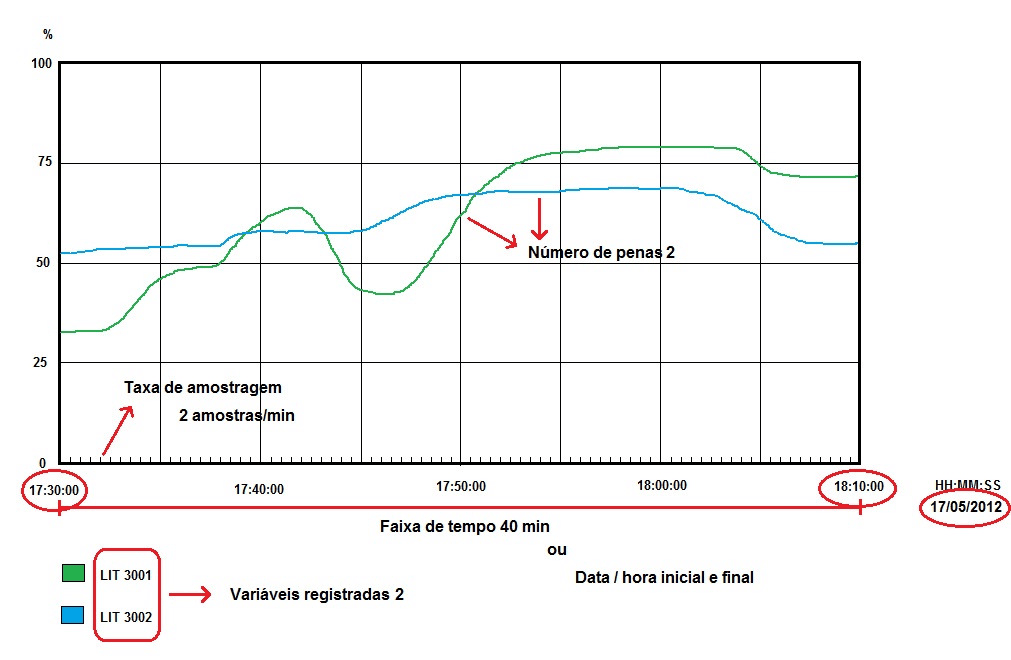
\includegraphics{../figuras/cap16-parametros-tendencia.png}
\caption[Figura 16.2 -- Parâmetros de configuração de um gráfico de tendência]{Figura 16.2 -- Parâmetros de configuração de um gráfico de tendência. \textbf{Fonte:} \emph{Livro SCADA --- versão para análise}, p.~70 (Machado, Pontes e Vianna, reproduzida com crédito).}
\end{figure}

\textbf{Tabela 16.2 -- Parâmetros do gráfico de tendência}

\begin{longtable}[]{@{}
  >{\raggedright\arraybackslash}p{(\columnwidth - 4\tabcolsep) * \real{0.3333}}
  >{\raggedright\arraybackslash}p{(\columnwidth - 4\tabcolsep) * \real{0.3333}}
  >{\raggedright\arraybackslash}p{(\columnwidth - 4\tabcolsep) * \real{0.3333}}@{}}
\toprule\noalign{}
\begin{minipage}[b]{\linewidth}\raggedright
Parâmetro
\end{minipage} & \begin{minipage}[b]{\linewidth}\raggedright
O que define
\end{minipage} & \begin{minipage}[b]{\linewidth}\raggedright
Consequência de errar
\end{minipage} \\
\midrule\noalign{}
\endhead
\bottomrule\noalign{}
\endlastfoot
Taxa de amostragem & Intervalo entre amostras gravadas & Subamostragem esconde o transitório (Capítulo 14) \\
Número de penas & Quantas variáveis na mesma escala & Acima de poucas penas, as cores deixam de ser distinguíveis \\
Variáveis registradas & Quais tags entram no vetor & Tag fora do vetor não tem histórico no período \\
Faixa de tempo e escala & Janela exibida e limites do eixo & Escala automática esconde comparação; escala fixa esconde a variação \\
\end{longtable}

\begin{caixadica}

\textbf{Dica:} escolha as variáveis de um mesmo gráfico pela \textbf{dinâmica}, não pela área da planta.
Misturar na mesma escala uma vazão que oscila a cada segundo com a temperatura de um tanque que
varia em horas produz um gráfico em que uma das curvas é uma linha reta --- e o operador aprende a
ignorá-la. Quando a comparação entre dinâmicas diferentes for necessária, use eixos separados.

\end{caixadica}

\begin{caixaatencao}

\textbf{Atenção:} a escala automática é confortável e enganosa. Ela sempre preenche a tela, fazendo
uma variação de 0,1 \% parecer uma oscilação dramática. Em painel de operação, escala fixa com
faixa conhecida é o padrão; escala automática é ferramenta de investigação, não de vigilância.

\end{caixaatencao}

\begin{center}\rule{0.5\linewidth}{0.5pt}\end{center}

\hypertarget{por-que-banco-relacional-nuxe3o-uxe9-historiador}{%
\section{Por que banco relacional não é historiador}\label{por-que-banco-relacional-nuxe3o-uxe9-historiador}}

Um banco de dados relacional resolve bem cadastro, venda, financeiro. Ele não foi projetado para o
padrão de carga da indústria, que tem três características incômodas:

\begin{enumerate}
\def\labelenumi{\arabic{enumi}.}
\tightlist
\item
  \textbf{Volume alto e previsível.} Uma planta com 5.000 tags coletadas a cada segundo produz
  432 milhões de pontos por dia --- cerca de 158 bilhões em um ano. Com 16 bytes por ponto, isso
  passa de 2 TB por ano em armazenamento bruto, sem contar índices.
\item
  \textbf{Escrita sequencial e contínua.} O padrão é \emph{append}: quase nunca se atualiza um ponto antigo.
  Um banco relacional com índices em todas as colunas paga caro por uma flexibilidade que não é
  usada.
\item
  \textbf{Consulta por intervalo e por série.} Quase toda pergunta é ``valores da variável X entre T1 e
  T2''. Isso é um \emph{range scan} sobre uma série temporal, não um \emph{join}.
\end{enumerate}

Um banco de dados de séries temporais (\emph{TSDB}) existe para esse padrão. O que ele faz de diferente:

\textbf{Tabela 16.3 -- O que um TSDB acrescenta ao banco convencional}

\begin{longtable}[]{@{}
  >{\raggedright\arraybackslash}p{(\columnwidth - 2\tabcolsep) * \real{0.5000}}
  >{\raggedright\arraybackslash}p{(\columnwidth - 2\tabcolsep) * \real{0.5000}}@{}}
\toprule\noalign{}
\begin{minipage}[b]{\linewidth}\raggedright
Recurso
\end{minipage} & \begin{minipage}[b]{\linewidth}\raggedright
Para que serve
\end{minipage} \\
\midrule\noalign{}
\endhead
\bottomrule\noalign{}
\endlastfoot
Índice temporal nativo & Consulta por intervalo sem varrer a tabela inteira \\
Compressão por série & Estabilidade do sinal vira compressão; rampa é gravada ponto a ponto \\
Agregação contínua (\emph{rollup}) & Pré-calcula média, mínimo e máximo por hora e por dia \\
Política de retenção & Reduz a resolução ou descarta o dado antigo automaticamente \\
Resolução de tempo nativa & Carimbo de tempo com precisão declarada e sem ambiguidade \\
\end{longtable}

O modelo de dados continua sendo o mesmo de sempre --- \textbf{série, tempo, valor e qualidade} ---, e é
exatamente o que o Capítulo 14 descreveu do lado do tag. O que muda é como esse modelo é armazenado
e consultado.

\begin{caixanota}

\textbf{Nota:} o ``melhor banco'' não existe. Existe o banco adequado ao volume, à janela de retenção,
ao ferramental de consulta e à competência da equipe que vai mantê-lo. Um historian embarcado no
próprio supervisório é a escolha certa para quem precisa de 30 dias de dado e já tem o software; um
TSDB em contêiner é a escolha certa para quem precisa integrar processo e nuvem com consulta
programável.

\end{caixanota}

\begin{center}\rule{0.5\linewidth}{0.5pt}\end{center}

\hypertarget{compressuxe3o-o-que-o-histuxf3rico-decide-esquecer}{%
\section{Compressão: o que o histórico decide esquecer}\label{compressuxe3o-o-que-o-histuxf3rico-decide-esquecer}}

Historiador sem compressão é caro; historiador com compressão mal configurada é pior que caro,
porque produz uma série que parece verdadeira e não é.

O mecanismo mais difundido é a \textbf{compressão por exceção}, também chamada de \emph{swinging door}: o
software só grava um novo ponto quando o valor se afasta do último ponto gravado mais do que uma
tolerância definida.

\begin{lstlisting}
Sinal estavel em 50,0 %  -> 1 ponto, mais um refresh periodico
Rampa de 0 a 100 %       -> pontos a cada desvio de tolerancia
Degrau instantaneo       -> gravado como degrau, se a tolerancia
                            for menor que o degrau

tolerancia de compressao = erro maximo da serie reconstruida
\end{lstlisting}

Daí decorrem três consequências que precisam estar no projeto:

\begin{itemize}
\tightlist
\item
  A \textbf{tolerância de compressão é o erro máximo} que a curva reconstruída terá em relação ao sinal
  real. Declará-la é obrigatório em qualquer análise que dependa de precisão.
\item
  Quanto \textbf{maior a tolerância, mais liso} o gráfico fica e menor o volume gravado --- o que é ótimo
  para tendência de longo prazo e péssimo para diagnosticar transitório.
\item
  A compressão é \textbf{irreversível}. O ponto descartado na gravação não volta.
\end{itemize}

\begin{caixaatencao}

\textbf{Atenção:} o pico é a primeira coisa que a compressão descarta, e é justamente o que a
engenharia procura quando investiga uma falha. Em variáveis ligadas a proteção, a tolerância de
compressão deve ser a menor possível, e vale avaliar o registro explícito de mínimo e máximo por
intervalo --- recurso que preserva a envoltória do sinal mesmo com poucos pontos gravados.

\end{caixaatencao}

\begin{center}\rule{0.5\linewidth}{0.5pt}\end{center}

\hypertarget{retenuxe7uxe3o-agregauxe7uxe3o-e-conformidade}{%
\section{Retenção, agregação e conformidade}\label{retenuxe7uxe3o-agregauxe7uxe3o-e-conformidade}}

Reter tudo para sempre não é política de arquivo: é ausência de política. A prática é \textbf{reduzir
resolução com o tempo}, mantendo a informação estatística do período.

\textbf{Tabela 16.4 -- Política de retenção por classe de dado}

\begin{longtable}[]{@{}
  >{\raggedright\arraybackslash}p{(\columnwidth - 8\tabcolsep) * \real{0.2000}}
  >{\raggedright\arraybackslash}p{(\columnwidth - 8\tabcolsep) * \real{0.2000}}
  >{\raggedright\arraybackslash}p{(\columnwidth - 8\tabcolsep) * \real{0.2000}}
  >{\raggedright\arraybackslash}p{(\columnwidth - 8\tabcolsep) * \real{0.2000}}
  >{\raggedright\arraybackslash}p{(\columnwidth - 8\tabcolsep) * \real{0.2000}}@{}}
\toprule\noalign{}
\begin{minipage}[b]{\linewidth}\raggedright
Classe
\end{minipage} & \begin{minipage}[b]{\linewidth}\raggedright
Exemplos
\end{minipage} & \begin{minipage}[b]{\linewidth}\raggedright
Resolução inicial
\end{minipage} & \begin{minipage}[b]{\linewidth}\raggedright
Retenção típica
\end{minipage} & \begin{minipage}[b]{\linewidth}\raggedright
Agregação
\end{minipage} \\
\midrule\noalign{}
\endhead
\bottomrule\noalign{}
\endlastfoot
Transitório e proteção & Chaves de intertravamento, primeira falha & Na origem, por exceção & Meses & Nenhuma: eventos vão para o registro de eventos \\
Processo rápido & Vazão, pressão & 1 s & Dias a semanas & Média, mínimo e máximo por minuto \\
Processo lento & Temperatura, nível de tanque & 5 a 60 s & Meses a anos & Média por hora e por dia \\
Indicadores de gestão & Produção, consumo, energia & 1 min ou por evento & Anos & Totais diários e mensais \\
\end{longtable}

Três cuidados completam a política:

\begin{itemize}
\tightlist
\item
  \textbf{Agregar preservando extremos.} Média por hora sem mínimo e máximo apaga o pico da hora --- e é
  exatamente o pico que interessa em consumo, vazão e temperatura.
\item
  \textbf{Backup com restauração testada.} Histórico que existe em um só disco não é histórico; é um
  arquivo temporário.
\item
  \textbf{Expurgo planejado.} O Livro SCADA de origem já alertava para a necessidade de critério de
  esvaziamento e \emph{backup} dos arquivos de registro, ``a fim de evitar ocupação total da mídia''. Em
  sistemas atuais, isso é resolvido pela própria política de retenção do banco, mas a decisão de
  quanto tempo guardar continua sendo da engenharia --- e frequentemente responde a exigências
  regulatórias e contratuais, não a preferências técnicas.
\end{itemize}

\begin{center}
\IfFileExists{../figuras/capitulo-16-m1.pdf}{%
  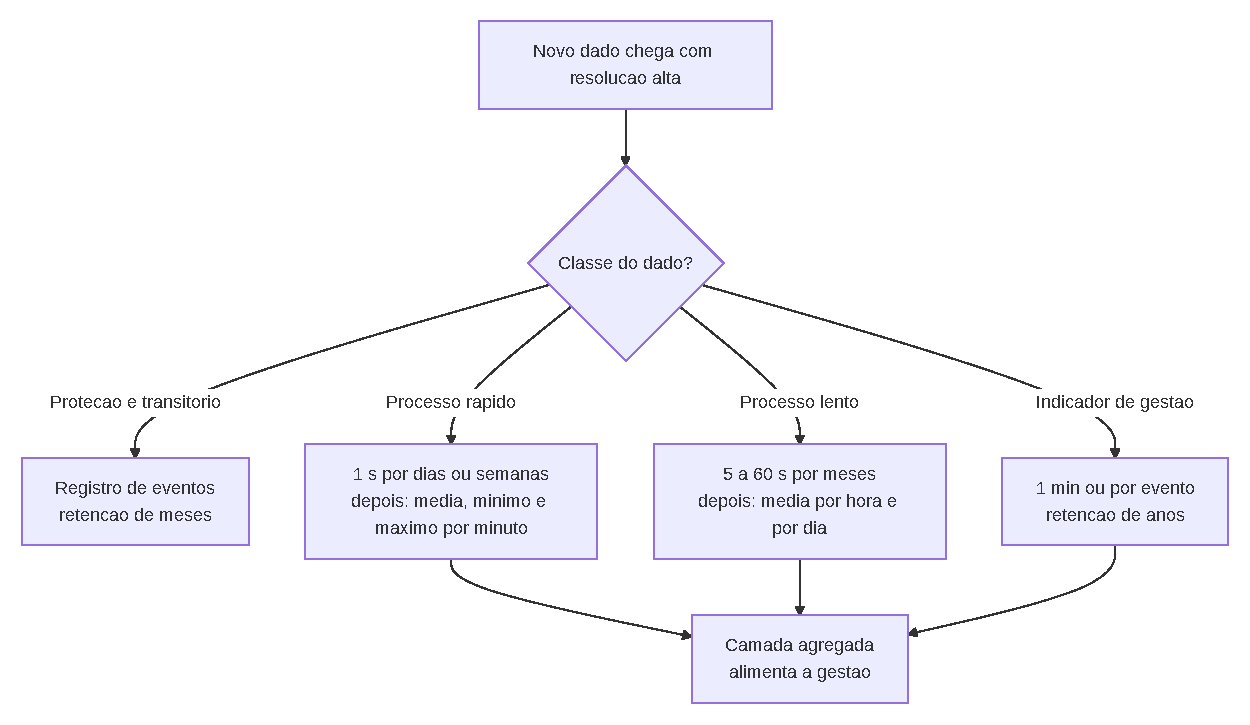
\includegraphics[width=\linewidth,height=0.8\textheight,keepaspectratio]{../figuras/capitulo-16-m1.pdf}%
}{\fbox{\parbox{0.9\linewidth}{\small Diagrama Mermaid ainda não renderizado: capitulo-16-m1. Rode scripts/render-mermaid.sh.}}}
\end{center}

\begin{caixafigura}

\textbf{{[}Figura 16.3 -- Consulta de histórico com agregação e comparação de períodos{]}}
\emph{Captura de uma tela de consulta a séries temporais com três controles visíveis: seleção de variáveis por ativo, intervalo de tempo (data e hora inicial e final) e função de agregação (média, mínimo, máximo, por hora ou por dia). O gráfico exibe duas curvas sobrepostas de períodos diferentes, com legenda identificando cada período e uma tabela resumida abaixo com mínimo, média e máximo de cada série. Destacar que a agregação está explícita na consulta e não escondida no painel.}

\end{caixafigura}

\begin{center}\rule{0.5\linewidth}{0.5pt}\end{center}

\hypertarget{histuxf3rico-de-processo-histuxf3rico-de-eventos}{%
\section{\texorpdfstring{Histórico de processo \ensuremath{\times} histórico de eventos}{Histórico de processo  histórico de eventos}}\label{histuxf3rico-de-processo-histuxf3rico-de-eventos}}

São dois registros, com dois propósitos, e misturá-los prejudica os dois.

\textbf{Tabela 16.5 -- Comparativo dos dois registros}

\begin{longtable}[]{@{}
  >{\raggedright\arraybackslash}p{(\columnwidth - 4\tabcolsep) * \real{0.3333}}
  >{\raggedright\arraybackslash}p{(\columnwidth - 4\tabcolsep) * \real{0.3333}}
  >{\raggedright\arraybackslash}p{(\columnwidth - 4\tabcolsep) * \real{0.3333}}@{}}
\toprule\noalign{}
\begin{minipage}[b]{\linewidth}\raggedright
Aspecto
\end{minipage} & \begin{minipage}[b]{\linewidth}\raggedright
Histórico de processo
\end{minipage} & \begin{minipage}[b]{\linewidth}\raggedright
Histórico de eventos e alarmes
\end{minipage} \\
\midrule\noalign{}
\endhead
\bottomrule\noalign{}
\endlastfoot
Conteúdo & Valor de variável ao longo do tempo & Ocorrência com carimbo, estado, prioridade e reconhecimento \\
Formato & Série temporal por tag & Lista cronológica de registros \\
Volume & Milhões de pontos por dia & Centenas a milhares de registros por dia \\
Consulta típica & ``Valores de X entre 14h e 15h'' & ``O que aconteceu entre 14h e 15h e quem reconheceu'' \\
Uso & Diagnóstico, otimização, relatório de processo & Investigação de causa, auditoria de operação, indicador de desempenho \\
\end{longtable}

A \textbf{trilha de auditoria} é um terceiro registro, ainda distinto: quem comandou, quem mudou
\emph{setpoint}, quem alterou limite de alarme, quem reiniciou o registrador de primeira falha. Esse
registro responde à pergunta ``quem fez'', que nem o histórico de processo nem a lista de eventos
respondem sozinhos --- e é requisito de qualquer sistema sujeito a auditoria (Capítulo 8).

\begin{center}
\IfFileExists{../figuras/capitulo-16-m2.pdf}{%
  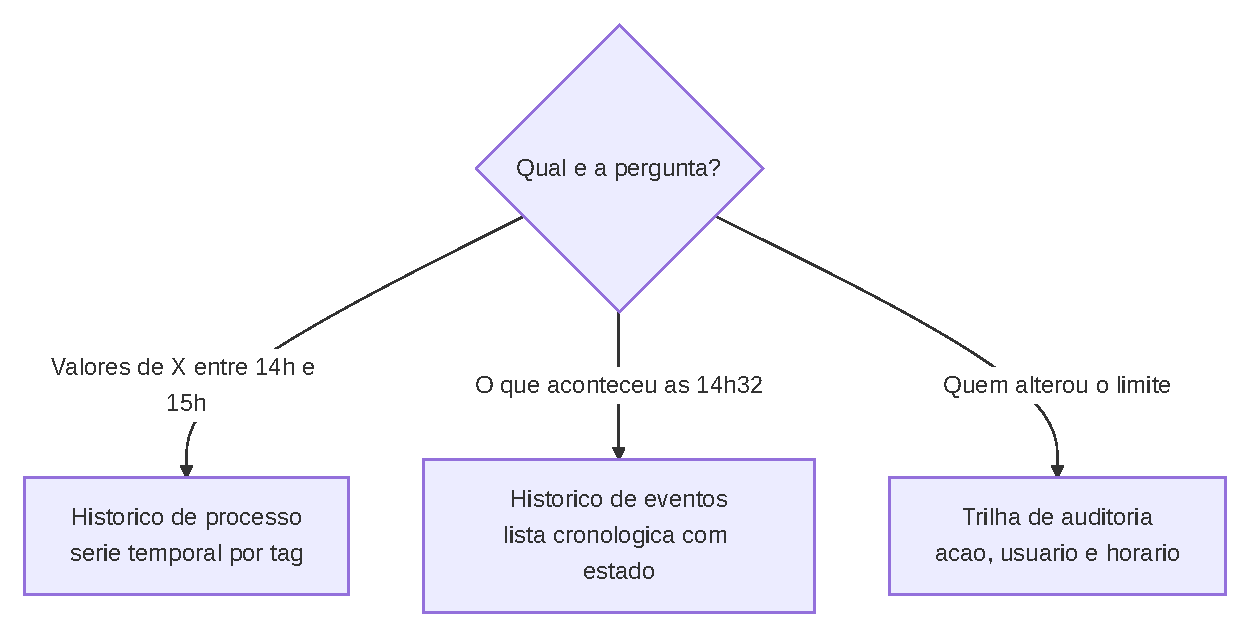
\includegraphics[width=\linewidth,height=0.8\textheight,keepaspectratio]{../figuras/capitulo-16-m2.pdf}%
}{\fbox{\parbox{0.9\linewidth}{\small Diagrama Mermaid ainda não renderizado: capitulo-16-m2. Rode scripts/render-mermaid.sh.}}}
\end{center}

\begin{caixadica}

\textbf{Dica:} antes de escolher um historian, escreva as cinco consultas que você precisa responder.
``Consumo diário por setor, últimos 12 meses'', ``todas as partidas da bomba 2 com duração acima de
30 s'', ``temperatura média e máxima do mancal na semana da falha''. A ferramenta que responde às suas
cinco consultas com o esforço aceitável é a ferramenta certa --- o resto é argumento de catálogo.

\end{caixadica}

\begin{center}\rule{0.5\linewidth}{0.5pt}\end{center}

\hypertarget{comparativo-das-soluuxe7uxf5es-de-historizauxe7uxe3o}{%
\section{Comparativo das soluções de historização}\label{comparativo-das-soluuxe7uxf5es-de-historizauxe7uxe3o}}

\textbf{Tabela 16.6 -- Famílias de solução}

\begin{longtable}[]{@{}
  >{\raggedright\arraybackslash}p{(\columnwidth - 10\tabcolsep) * \real{0.1667}}
  >{\raggedright\arraybackslash}p{(\columnwidth - 10\tabcolsep) * \real{0.1667}}
  >{\raggedright\arraybackslash}p{(\columnwidth - 10\tabcolsep) * \real{0.1667}}
  >{\raggedright\arraybackslash}p{(\columnwidth - 10\tabcolsep) * \real{0.1667}}
  >{\raggedright\arraybackslash}p{(\columnwidth - 10\tabcolsep) * \real{0.1667}}
  >{\raggedright\arraybackslash}p{(\columnwidth - 10\tabcolsep) * \real{0.1667}}@{}}
\toprule\noalign{}
\begin{minipage}[b]{\linewidth}\raggedright
Tecnologia
\end{minipage} & \begin{minipage}[b]{\linewidth}\raggedright
Função
\end{minipage} & \begin{minipage}[b]{\linewidth}\raggedright
Protocolo ou interface
\end{minipage} & \begin{minipage}[b]{\linewidth}\raggedright
Aplicação
\end{minipage} & \begin{minipage}[b]{\linewidth}\raggedright
Vantagens
\end{minipage} & \begin{minipage}[b]{\linewidth}\raggedright
Limitações
\end{minipage} \\
\midrule\noalign{}
\endhead
\bottomrule\noalign{}
\endlastfoot
Historizador do próprio supervisório & Série temporal integrada à aplicação de supervisão & Nativo, OPC DA/UA & Planta única, escopo de operação & Já integrado, sem projeto de infraestrutura & Retenção e consulta limitadas; integração externa mais difícil \\
Historizador de processo dedicado & Série temporal industrial em escala de planta e corporação & OPC DA/UA, HDA, API própria & Múltiplas plantas, indicadores corporativos & Compressão madura, consulta rápida, ferramental consolidado & Licença por ponto; projeto longo \\
Banco de séries temporais de código aberto & Série temporal com consulta por linguagem própria & HTTP, linha de comando, \emph{drivers} & Integração com dashboards e nuvem & Custo de licença baixo, integração ampla, retenção configurável & Exige operação de infraestrutura e disciplina de modelagem \\
Plataforma IIoT & Série temporal com entidades, alarmes e regras & MQTT, HTTP, REST & Frota de dispositivos e telemetria & Já traz alarme, painel e gestão de dispositivos & Modelo de dados próprio; histórico de alta resolução exige configuração \\
Arquivo plano (CSV, registrador de carta digital) & Registro simples para conferência & Arquivo & Bancada, ensaio pontual, laudo & Simples e portátil & Sem consulta, sem índice, sem escala \\
\end{longtable}

A combinação mais comum em projetos atuais é \textbf{duas camadas}: o historian junto ao processo, com
alta resolução e escopo curto, e um TSDB ou plataforma na camada de integração, com resolução
reduzida e retenção longa. As duas camadas não se substituem --- a primeira responde ao diagnóstico, a
segunda responde à gestão.

\begin{center}\rule{0.5\linewidth}{0.5pt}\end{center}

\hypertarget{estudo-de-caso-o-pico-que-o-histuxf3rico-nuxe3o-viu}{%
\section{\texorpdfstring{Estudo de Caso --- O pico que o histórico não viu}{Estudo de Caso  O pico que o histórico não viu}}\label{estudo-de-caso-o-pico-que-o-histuxf3rico-nuxe3o-viu}}

\textbf{Cenário.} Uma estação de bombeamento registrava a pressão de recalque em um historian configurado
com taxa de amostragem de 30 s e tolerância de compressão de 2 \% da faixa. Em três meses, dois
motores falharam por sobrecarga em partida. A investigação pediu as curvas de pressão dos dez
minutos que antecederam cada partida --- e encontrou uma reta.

\textbf{Diagnóstico.} Quatro decisões de projeto, tomadas em momentos diferentes, se somaram:

\begin{enumerate}
\def\labelenumi{\arabic{enumi}.}
\tightlist
\item
  A taxa de 30 s foi escolhida quando o historian ainda rodava em um servidor antigo, para caber no
  disco. A limitação deixou de existir, a configuração ficou.
\item
  A tolerância de compressão de 2 \% era adequada para relatório mensal e destruía o transitório de
  partida, que dura entre 3 e 8 segundos.
\item
  A variável estava no grupo de amostragem lenta do driver, com 10 s de varredura --- os primeiros
  segundos da partida nunca chegavam ao historian.
\item
  Não havia registro de mínimo e máximo por intervalo, o que teria preservado ao menos a envoltória
  do pico.
\end{enumerate}

\textbf{Decisão de engenharia.}

\begin{longtable}[]{@{}
  >{\raggedright\arraybackslash}p{(\columnwidth - 2\tabcolsep) * \real{0.5000}}
  >{\raggedright\arraybackslash}p{(\columnwidth - 2\tabcolsep) * \real{0.5000}}@{}}
\toprule\noalign{}
\begin{minipage}[b]{\linewidth}\raggedright
Medida
\end{minipage} & \begin{minipage}[b]{\linewidth}\raggedright
Efeito
\end{minipage} \\
\midrule\noalign{}
\endhead
\bottomrule\noalign{}
\endlastfoot
Pressão de recalque e corrente do motor migradas para grupo rápido (1 s) no driver & O transitório passa a ser observável \\
Tolerância de compressão reduzida para 0,2 \% nas variáveis de processo crítico & O pico deixa de ser descartado \\
Ativação do registro de mínimo e máximo por minuto & A envoltória é preservada mesmo no dado antigo \\
Cópia agregada (média, mínimo, máximo por hora) para a camada de gestão & Retenção longa sem custo de armazenamento alto \\
\end{longtable}

\textbf{Resultado.} A terceira partida monitorada mostrou elevação de pressão de 40 \% acima do normal nos
primeiros 4 segundos, seguida de fechamento lento da válvula de retenção --- a mesma causa identificada
no estudo de caso do Capítulo 15, agora visível na curva.

\textbf{Limitações do arranjo.} A mudança não recupera o histórico já comprimido: os dois primeiros
eventos continuarão sem explicação no dado. E o aumento de resolução tem custo de armazenamento que
precisa ser dimensionado --- a solução não é migrar tudo para 1 s, e sim escolher as variáveis em que
o transitório tem significado.

\begin{center}\rule{0.5\linewidth}{0.5pt}\end{center}

\hypertarget{resumo}{%
\section{Resumo}\label{resumo}}

\begin{itemize}
\tightlist
\item
  O histórico atende \textbf{operação, engenharia e gestão}, com exigências de resolução e retenção que não coincidem.
\item
  \textbf{Tendência real} vive em memória e tem janela limitada pelo vetor; \textbf{tendência histórica} vive em disco e responde por período.
\item
  A janela da tendência real é o produto da taxa de amostragem pelo número de amostras: não há como ampliar as duas ao mesmo tempo.
\item
  Banco relacional não é historian por causa do volume, do padrão de escrita sequencial e do tipo de consulta.
\item
  \textbf{Compressão por exceção} define o erro máximo da série reconstruída e é irreversível: o pico é o primeiro dado a ser descartado.
\item
  Política de retenção deve \textbf{reduzir resolução com o tempo}, preservando mínimo e máximo nas agregações.
\item
  Histórico de processo, histórico de eventos e trilha de auditoria são três registros distintos.
\item
  A escolha da ferramenta sai das \textbf{cinco consultas} que o projeto precisa responder.
\end{itemize}

\hypertarget{questuxf5es-de-revisuxe3o}{%
\section{Questões de Revisão}\label{questuxf5es-de-revisuxe3o}}

\begin{enumerate}
\def\labelenumi{\arabic{enumi}.}
\tightlist
\item
  Explique a diferença entre tendência real e tendência histórica quanto a armazenamento, comportamento e uso.
\item
  Uma tendência real tem vetor de 2.048 amostras. Qual a janela de tempo com taxa de 500 ms e com taxa de 5 s? Que compromisso você está fazendo em cada caso?
\item
  Por que um banco de dados relacional não é a escolha adequada para historização de processo? Cite as três características do padrão de carga industrial.
\item
  Estime o volume anual de pontos de um sistema com 2.000 tags gravadas a cada 2 s e discuta se o armazenamento bruto é aceitável.
\item
  Explique o que é compressão por exceção e por que a tolerância de compressão é o erro máximo da série reconstruída.
\item
  Uma variável de proteção e uma temperatura ambiente serão historizadas. Proponha taxa de amostragem, tolerância de compressão e retenção para cada uma, justificando.
\item
  Descreva uma política de retenção em três camadas para uma planta de saneamento, indicando o que se guarda em cada camada e por quanto tempo.
\item
  Qual a diferença entre histórico de processo, histórico de eventos e trilha de auditoria? Dê um exemplo de pergunta que só a trilha de auditoria responde.
\item
  Um operador afirma que ``a pressão nunca passou de 8 bar'' e a engenharia mede 11 bar com um registrador independente. Que decisões de configuração do historian podem explicar a divergência?
\end{enumerate}

\hypertarget{referuxeancias}{%
\section{Referências}\label{referuxeancias}}

\begin{itemize}
\tightlist
\item
  MACHADO, R.; PONTES, W.; VIANNA, W. \textbf{Livro SCADA --- versão para análise}. Material didático do curso (seções sobre gráficos de tendência real e histórica, parâmetros de configuração, relatórios e esvaziamento de arquivos de registro). Figuras reproduzidas com crédito.
\item
  VIANNA, W. S. \textbf{Sistema SCADA Supervisório}. IFF, 2008 (seções sobre gráficos de tendência e gerador de relatórios).
\item
  INFLUXDATA. \textbf{InfluxDB Documentation} --- modelo de dados, políticas de retenção e tarefas de agregação contínua. Disponível em: docs.influxdata.com. Consulta: 2026.
\item
  TIMESCALE. \textbf{TimescaleDB Documentation} --- hipertabelas, compressão e agregação contínua sobre PostgreSQL. Disponível em: docs.timescale.com. Consulta: 2026.
\item
  GRAFANA LABS. \textbf{Grafana Documentation} --- consulta a séries temporais, agregação na consulta e painéis. Disponível em: \url{grafana.com/docs}. Consulta: 2026.
\item
  OPC FOUNDATION. \textbf{OPC UA Part 11 --- Historical Access}: leitura de histórico no próprio servidor (\passthrough{\lstinline!HistoryRead!}). Disponível em: opcfoundation.org. Consulta: 2026.
\item
  AVEVA. \textbf{PI System} --- visão geral de historização industrial e compressão de séries temporais. Disponível em: aveva.com. Consulta: 2026 (citado por função, sem comparativo de produto).
\end{itemize}
